\chapter{Hashfunktionen}
Bei einer Hashfunktion ist die Wertemenge meist wesentlich kleiner als die Lösungsmenge. \\
Die Elemente der Wertmenge können normalerweise eine beliebige Länge haben. \\
Die Elemente der Lösungsmenge haben meist eine fixe Länge.

\begin{tabbing}
	$\bullet$ Anfangsbuchstabe: ~~~~ \= Hallo $\rightarrow$ H \\
	~~~~~~~~~~~~~~~~~~~~~~~~~~~~~~~~ \= Tim $\rightarrow$ T \\
	$\bullet$ Postleitzahl: ~~~~~ \= Grins $\rightarrow$ 6591 \\
	~~~~~~~~~~~~~~~~~~~~ \= Neustift $\rightarrow$ 6167 \\
	$\bullet$ CRC ...
\end{tabbing}

\section{Kryptographische Hashfunktionen}
Kryptographische Hashfunktionen müssen spezielle Eigenschaften erfüllen. Die wichtigste Eigenschaft ist, dass es sich um eine Einwegfunktion handelt.
\begin{figure}[H]
	\centering
	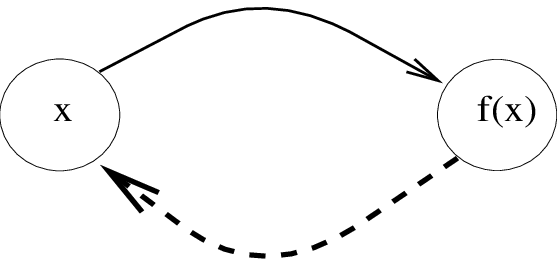
\includegraphics[width=0.6\linewidth]{figures/oneway.png}
	\caption{Einwegfunktion}
\end{figure}

\subsection*{Eigenschaften}
\begin{itemize}
	\item \textbf{Einwegfunktion:} Unumkehrbarkeit muss so gut wie möglich gegeben sein
	\item Diffusion ('Lawineneffekt'): kleine Änderung in der Eingabe bewirkt die ganze Ausgaben.
	\item Konfusion: Von Hashwert kann man keine Rückschlüsse auf den Eingabewert machen
	\item Eindeutigkeit
	\item Kollisionsresistenz: Die Wahrscheinlichkeit, dass Kollisionen vorkommen soll so klein wie möglich sein (im besten Fall gleich Null sein)
\end{itemize}

\subsection*{Hash-Algorithmen}
\begin{itemize}
	\item MD5: 128 Bit Hashwert, unsicher!
	\item SHA (secure hash algorithm)
	\begin{itemize}
		\item SHA1: 160 Bit Hashwerte unsicher!
		\item SHA2 \\
		$\rightarrow$ SHA224, SHA256, SHA 384, SHA512
		\item SHA3: grundlegend anders, 224, 256, 384 Bitwerte $\rightarrow$ auch frei wählbar
	\end{itemize}
	\item GOST, Whirlpool
\end{itemize}

\subsection*{Ablauf SHA-256} 
\begin{itemize}
	\item Block erstellen (Auffüllen, Startblock erstellen, Wurzel von Primzahlen)
	\item Bitrotation, Zeilen integrieren (Diffusion)
	\item XOR, Bitshift (viele Runden)
	\item Auswahlfunktion, Mehrheitsfunktion (Einwegfunktion)
\end{itemize}

\textbf{Zusatz:} Message Authentication Code z.B. HMAC: Schlüssel-Hash-Nachtrichtauthentifizierung, Pre-Shared-Key

\subsection*{Angriffe}
\begin{itemize}
	\item Brute-Force
	\item Phising
	\item Wörterbuchangriff
	\item Algorithmus mutzen
	\item Rainbow-Table (viel Speicher) \\
	$\rightarrow$ viele Hashwerte als Kette gespeichert
\end{itemize}

\section{Passwörter}
\begin{enumerate}
	\item \textbf{lokale Speicherung}
	\begin{itemize}
		\item Länge des Passworters (mind 12 Zeichen)
		\item keine Wörter, persönliche Informationen
		\item Buchstaben/Zahlen/Symbole
		\item Jedes Passwort nur einmal verwenden
		\item Passwortmanager verwenden oder MFA als Alternative
	\end{itemize}
	\item \textbf{Speicherung am Server}
	\begin{itemize}
		\item \textbf{Klartext} \Lightning: Zugriff auf Datenbank, Admin, MITM
		\item \textbf{Gehashed} \Lightning: MITM, gleiche Passwörter erkennbar
		\item \textbf{Gehashed + Salt:} Mitm, Brute-Force
		\item \textbf{Gehashed + Salt + Pepper} \\
		\textbf{Salt:} Zufällige Zeichenkette die im Klartext in der Datenbank gespeichert wird $\rightarrow$ Jeder bekommt eigenen Hashwert \\
		\textbf{Pepper:} Zufällige Zeichenkette die NICHT in der Datenbank steht
	\end{itemize}
	\item \textbf{Austausch Client-Server}
	\begin{itemize}
		\item PAP unsicher! 
		\begin{figure}[H]
			\centering
			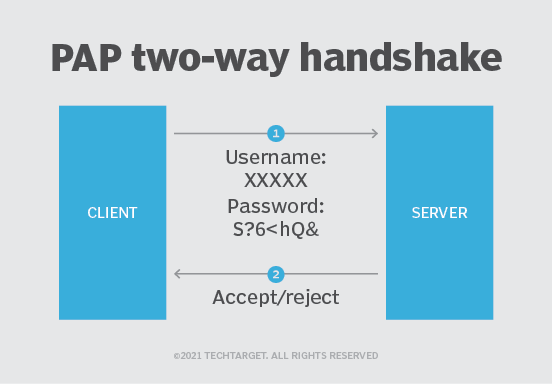
\includegraphics[width=0.6\linewidth]{figures/pap.png}
			\caption{PAP}
		\end{figure}
		\item CHAP: Bei CHAP wird bei jedem Anmeldeversuch eine Challenge (Zufallszahl) gesendet. Der Client hashed sein Passwort mit der Zufallszahl und sendet es dem Server. Der Server kann dann das Passwort in der Datenbank mit der gesendeten Zufallszahl hashen und es mit dem Client-Hash vergleichen. Somit wird zum einem, das Passwort nie im Klartext gesendet und zum anderen kann der gesendete Hash nicht nocheinmal gesendet werden, da die Zufallszahl 'einzigartig' ist und bei jedem Anmeldeversuch anders ist. \\
		$\rightarrow$ MITM Anmeldung mit dem Hashwert ist durch die Challenge nicht mehr möglich
		\begin{figure}[H]
			\centering
			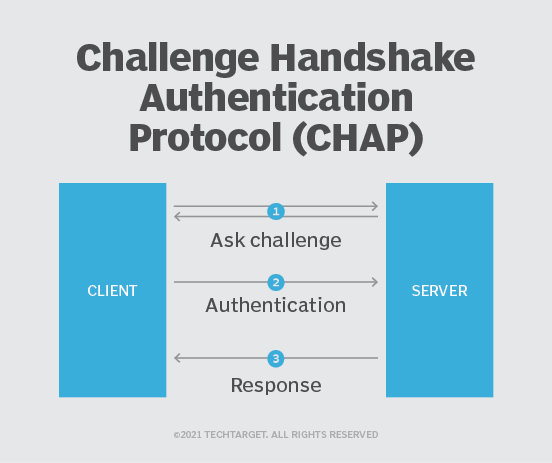
\includegraphics[width=0.6\linewidth]{figures/chap.png}
			\caption{PAP}
		\end{figure}
		\textbf{Alternativen:} MS-CHAPv1, MSCHAPv2, EAP, PEAP,...
	\end{itemize}
\end{enumerate}

\section{AAA}
Autorisierung (Was?), Authentifizierung (Wer?) \& Accounting (Wann?) \\
Protokolle: RADIUS, TACACS+

\section{PKI (Public Key Infrastruktur)}
Digitale Zertifikate sind für die Authentifizierung eines öffentlichen Schlüssels und seiner zulässigen Anwendung bzw. Geltungsbereich 

\begin{tabbing}
	Vergleich: ~~~~~~~~ \= Zertifikat $\rightarrow$ Pass \\
	~~~~~~~~~~~~ \= digitale Signatur $\rightarrow$ Foto
\end{tabbing}

\begin{figure}[H]
	\centering
	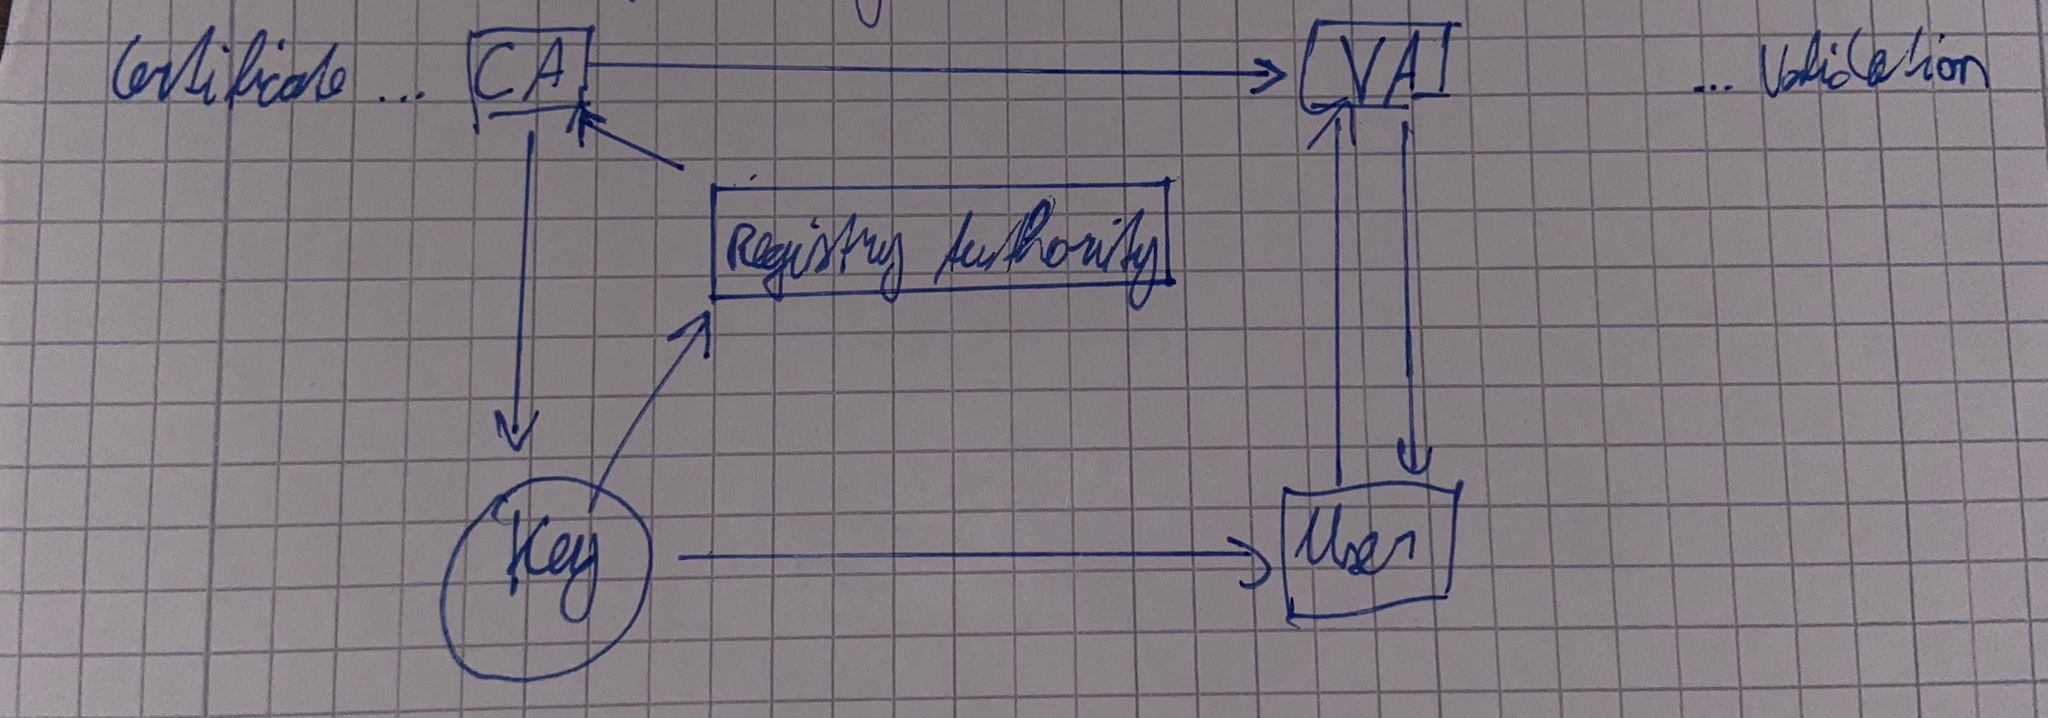
\includegraphics[width=0.7\linewidth]{figures/cert.jpeg}
	\caption{Public Key Infrastruktur}
\end{figure}

\textbf{Alternative:} Web of Trust \\

\section{Zusammenfassung}
\begin{tabular}{ | p{\dimexpr 0.5\linewidth-2\tabcolsep} | p{\dimexpr 0.5\linewidth-2\tabcolsep} |} \hline
	\textbf{verwendete Algorithmen} & \textbf{typische Protokolle} \\ \hline
	AES/DES & HTTPS \\
	RSA & IPsec \\
	Diffie-Hellman & VPN \\
	Hashfunktionen (SHA256,...) & SSH \\
	MAC (bzw. HMAC) & PSK (WLAN) \\
	Authentifizierung (AAA, CHAP) & RADIUS \\
	PKI & ... \\
	\hline
\end{tabular} 

\section{HTTPS} 
HTTP + TLS (SSL) \\
TLS ... transport layer security, Verschlüsselung nach Layer 4
\begin{itemize}
	\item Symmetrische Verschlüsselung
	\item Asymmetrischer Schlüsselaustausch (ab TLS 1.3 Diffie-Hellman)
	\item Authentifizierung (Server), PKI, RSA
	\item Hashfunktionen (SHA256,...)
	\item Sicherung der Nachrichtenintegrität (HMAC)
\end{itemize}

\begin{figure}[H]
	\centering
	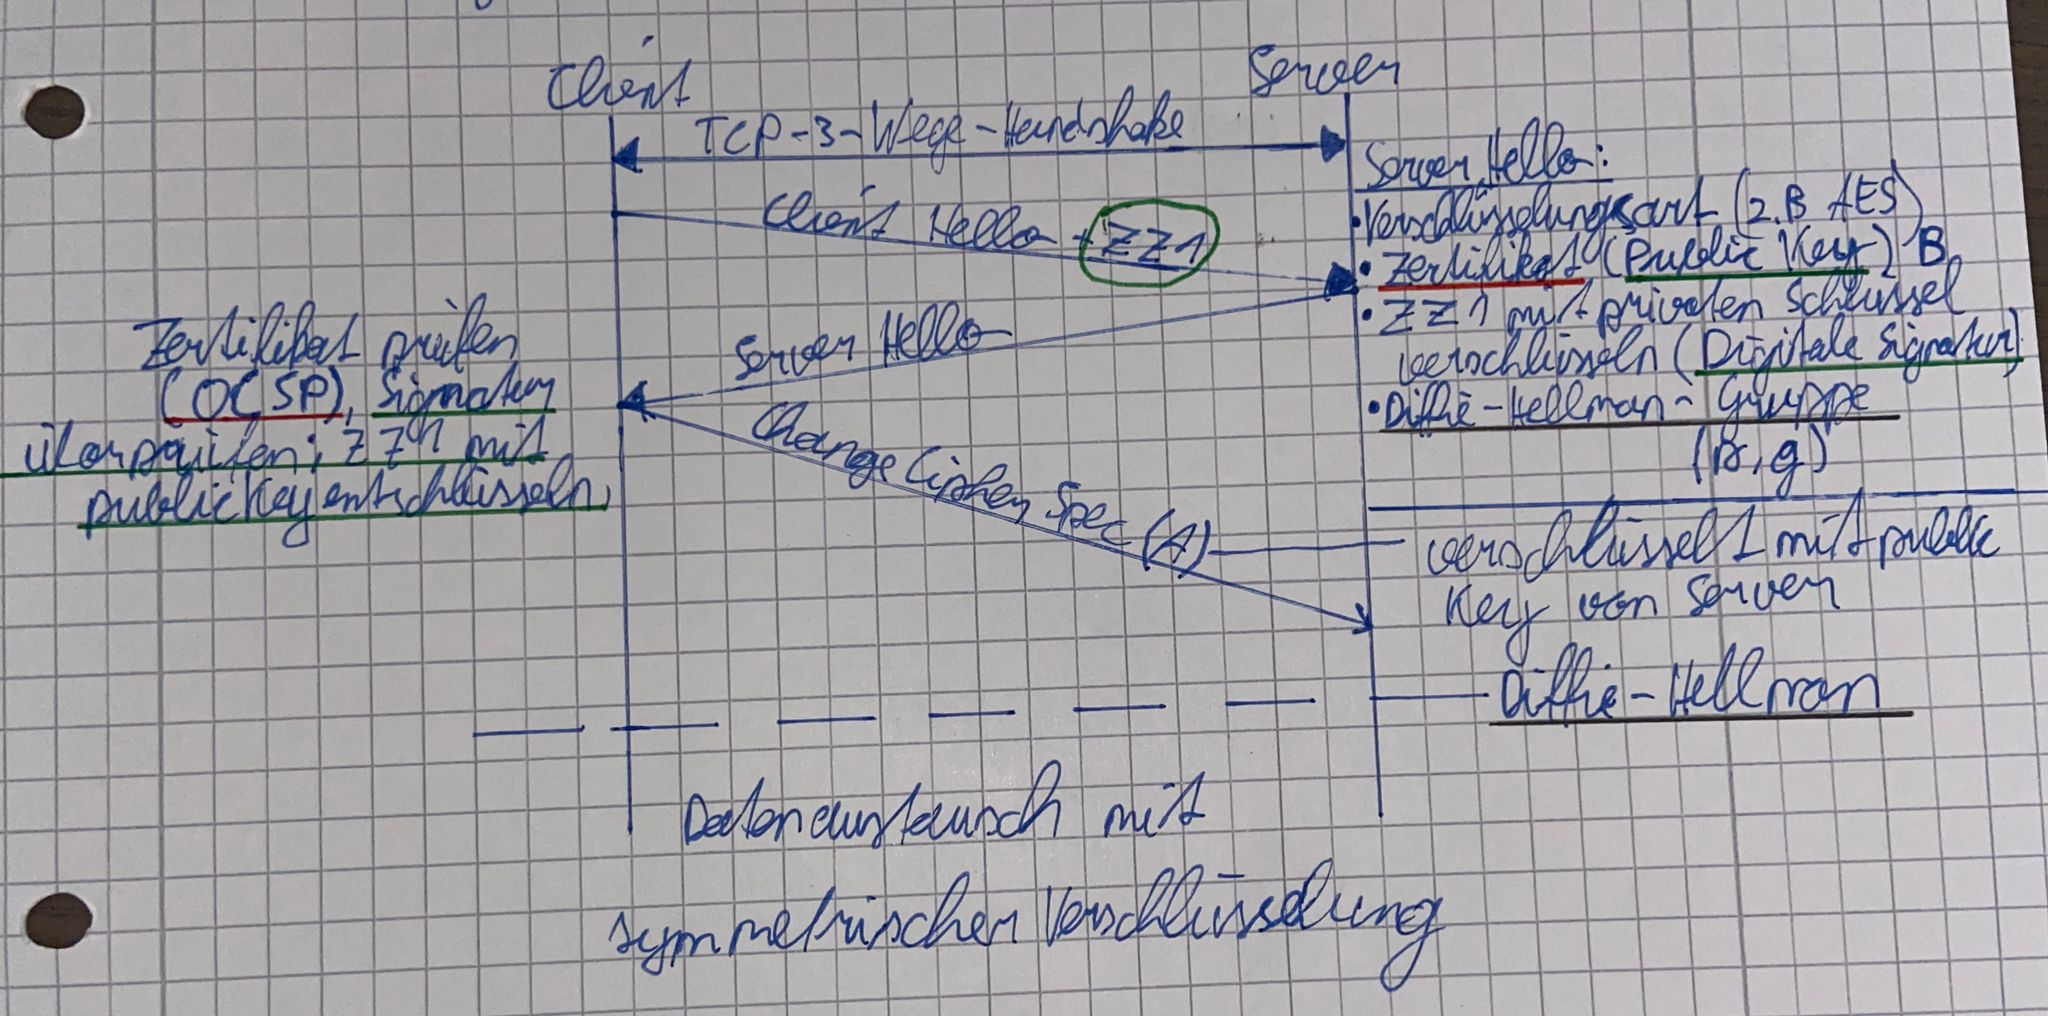
\includegraphics[width=1.0\linewidth]{figures/https.jpeg}
	\caption{HTTPS Verbindungsaufbau}
\end{figure}









